\section{Introduction}\label{sec:intro}

Population health research is becoming increasingly based on data-driven methods
(as opposed to those designed solely by clinical experts) for patient-centred
care through the advent of accessible software and a relative abundance of
electronic data. Population health research concerns itself with better
understanding the healthcare needs and behaviours of a population, so to further
that end it can be helpful to find an appropriate segmentation of that
population; such a segmentation allows for finer-grained analysis of groups in
the population that share some form of homogeneity. One commonly used method for
such patient-centred analysis is that of patient flow and their interaction with
the healthcare system.

However, this process relies heavily on detailed data --- about both the system
and the population within that system --- which may limit research where
sophisticated data pipelines are not yet in place. This work demonstrates how
this issue may be overcome using administrative, spell-level hospital data to
build a useful patient clustering that feeds into a multi-class queuing model.
Specifically, this work examines patient records from the NHS Wales Cwm Taf
Morgannwg University Health Board (UHB) that present chronic obstructive
pulmonary disease (COPD). COPD is of particular interest to Cwm Taf Morgannwg as
the condition is known to often present as a comorbidity in
patients~\cite{Houben2019} and it was found that they had the highest prevalence
of the condition across all the Welsh health boards in an internal report by NHS
Wales.

% TODO No reference for graph sent by Kendal but is this alright?

% TODO Image of process: administrative data -> extract service parameters ->
%                        validate parameters with Wasserstein distance ->
%                        continue with queuing model as normal

\subsection{Literature review}\label{subsec:review}

Given the subject matter of this work, the relevant literature spans much of
operational research in healthcare and the focus of this review is on the
principal topics of segmentation analysis, the handling of missing or incomplete
data in healthcare settings and queuing theory applied to hospital systems.

\subsubsection{Segmentation analysis}

Segmentation analysis allows for the targeted analysis of otherwise
heterogeneous datasets and encompasses several techniques from operational
research, statistics and machine learning. One of the most desirable qualities
of this kind of analysis is the ability to glean and communicate simplified
summaries of patient needs to stakeholders within a healthcare
system~\cite{Vuik2016b, Yoon2020}. For instance, clinical profiling often
forms part of the wider analysis where each segment can be summarised in a
phrase or infographic~\cite{Vuik2016a, Yan2019}.

The review for this work identified three commonplace groups of patient
characteristics used to segment a patient population: their system
utilisation metrics, their clinical attributes and their pathway. The latter
is not used to segment the patients directly but rather groups their movements
through a healthcare system. This is typically done via process
mining.~\cite{Arnolds2018}~and~\cite{Delias2015} demonstrate how this technique
can be used to improve the efficiency of a hospital system as opposed to
tackling the more relevant issue of patient-centred care. The remaining
characteristics can be segmented with a number of techniques but recent works
tend to use unsupervised methods, typically latent class analysis (LCA) or
clustering~\cite{Yan2018}.

LCA is a statistical, model-based method used to identify groups (called latent
classes) in data by relating its observations to some unobserved (latent),
categorical attribute. This attribute has multiple categories, each
corresponding to a latent class. The discovered relations are then used to
separate the observations into latent classes according to their maximum
likelihood class membership~\cite{Hagenaars2002,Lazarsfeld1968}. This method has
proved useful in the study of comorbidity patterns as
in~\cite{Larsen2017,Kuwornu2014} where combinations of demographic and clinical
attributes are related to various subgroups of chronic diseases.

Similarly to LCA, clustering identifies groups (clusters) in data to produce a
labelling of its instances. However, clustering includes a wide variety of
methods where the common theme is to maximise homogeneity within, and
heterogeneity between, each cluster~\cite{Everitt2011}. The \(k\)-means paradigm
is the most popular form of clustering in literature. The method iteratively
partitions numerical data into \(k \in \mathbb{N}\) distinct parts where \(k\)
is fixed \emph{a priori}. This method has proved popular as it is easily
scalable and its implementations are concise~\cite{Olafsson2008,Wu2009}. In
addition to \(k\)-means, hierarchical clustering methods can be effective if a
suitable number of parts cannot be found initially~\cite{Vuik2016a}. Although,
supervised hierarchical segmentation methods such as classification and
regression trees (as in~\cite{Harper2006}) have been used where an existing,
well-defined label is of particular significance.

\subsubsection{Handling incomplete data}

This is a reference for the estimation of service times
(theoretically)~\cite{Goldenshluger2016,Kumar2010}.

\subsubsection{Queuing models}

These are the principal queuing theory works by
Erlang~\cite{Erlang1917,Erlang1920}. This is a reference for the approximation
of general service times using phase-type distributions in single-server
queues~\cite{Djabali2018}. Deadlock is an aspect of applied queuing theory of
interest in recent literature~\cite{Palmer2018}. The software used is
Ciw~\cite{Palmer2019}.

% TODO Brief literature review of:
%       - reverse-engineering model parameters in healthcare ???
%       - queuing in healthcare

\subsection{Overview of the dataset}\label{subsec:overview}

The dataset used in this work was provided by the Cwm Taf Morgannwg UHB as part
of an ongoing research project with the authors. The dataset contains a
spell-level summary of 5,243 patients presenting COPD from February 2011 through
March 2019 totalling 10,881 spells. 

\subsection{Cluster analysis}\label{subsec:clusters}

\begin{table}
    \centering
    \resizebox{\textwidth}{!}{%
        \begin{tabular}{lllllll}
\toprule
               &        &   Cluster &             &            &           & Population \\
               &        &         0 &           1 &          2 &         3 &            \\
\midrule
\textbf{Characteristics} & \textbf{Percentage of spells} &   9.90701 &     19.2708 &    69.3859 &   1.43633 &        100 \\
               & \textbf{Mean spell cost, £} &   8051.23 &     2309.63 &    1508.41 &   17888.4 &     2265.4 \\
               & \textbf{Percentage of recorded costs} &   29.0137 &     19.3806 &    48.2048 &   3.40094 &        100 \\
               & \textbf{Mean COPD adm. in last year} &   2.19331 &     1.96464 &     1.8819 &   2.08974 &    1.93168 \\
               & \textbf{Minimum LOS} &   12.8229 & -0.00486111 & -0.0208333 &   48.8174 & -0.0208333 \\
               & \textbf{Mean LOS} &   25.3024 &     6.46379 &    4.10628 &   75.3601 &    7.68393 \\
               & \textbf{Maximum LOS} &   51.3604 &      30.859 &     16.941 &   224.928 &    224.928 \\
               & \textbf{Median no. of LTCs} &         2 &           3 &          1 &         3 &          1 \\
               & \textbf{Median no. of ICDs} &         9 &           8 &          5 &        11 &          6 \\
               & \textbf{Median CCI} &         9 &          20 &          4 &        18 &          4 \\
\textbf{Intervention prevalence} & \textbf{None, \%} &   80.2045 &     83.4209 &    65.7643 &   89.7436 &    70.9419 \\
               & \textbf{PR, \%} &   15.7993 &     13.4257 &    27.9724 &   8.97436 &    23.6903 \\
               & \textbf{SN, \%} &   3.81041 &      2.8667 &     4.6311 &   1.28205 &    4.16168 \\
               & \textbf{Both, \%} &  0.185874 &     0.28667 &    1.63217 &         0 &    1.20615 \\
\textbf{LTC prevalence} & \textbf{Pulmonary disease, \%} &       100 &         100 &        100 &       100 &        100 \\
               & \textbf{Diabetes, \%} &    19.052 &     28.1414 &    14.8355 &        25 &    17.9634 \\
               & \textbf{AMI, \%} &   13.8476 &     22.9336 &    8.75796 &   16.0256 &    12.0983 \\
               & \textbf{CHF, \%} &   12.4535 &     53.8462 &          0 &   26.2821 &    11.9878 \\
               & \textbf{Renal disease, \%} &   7.52788 &     19.5413 &     1.9241 &   17.9487 &    6.10441 \\
               & \textbf{Cancer, \%} &   7.62082 &     12.2312 &    2.93259 &   10.8974 &    5.30338 \\
               & \textbf{Dementia, \%} &   6.87732 &     21.2613 &          0 &   26.9231 &    5.16527 \\
               & \textbf{CVA, \%} &   8.64312 &     13.3301 &   0.703291 &   19.8718 &    4.19851 \\
               & \textbf{PVD, \%} &   4.36803 &     7.69231 &    2.26911 &   5.76923 &    3.57242 \\
               & \textbf{CTD, \%} &   5.11152 &     4.25227 &     3.1051 &   4.48718 &    3.54479 \\
               & \textbf{Obesity, \%} &   2.50929 &     3.01003 &     1.4862 &   7.69231 &    1.97035 \\
               & \textbf{Metastatic cancer, \%} &   1.57993 &     4.49116 &          0 &  0.641026 &    1.03121 \\
               & \textbf{Paraplegia, \%} &   1.30112 &     3.72671 &   0.238854 &  0.641026 &    1.02201 \\
               & \textbf{Diabetic compl., \%} &  0.185874 &     0.86001 &   0.477707 &   1.92308 &   0.543228 \\
               & \textbf{Peptic ulcer, \%} &   1.57993 &    0.812231 &   0.225584 &   1.28205 &   0.487985 \\
               & \textbf{Sepsis, \%} &    1.7658 &    0.907788 &   0.145966 &   1.92308 &   0.478777 \\
               & \textbf{Liver disease, \%} &   0.27881 &    0.477783 &   0.225584 &         0 &   0.276218 \\
               & \textbf{C. diff, \%} &  0.743494 &   0.0955566 &  0.0132696 &  0.641026 &   0.110487 \\
               & \textbf{Severe liver disease, \%} &  0.185874 &    0.430005 &          0 &         0 &    0.10128 \\
               & \textbf{MRSA, \%} &   0.27881 &   0.0477783 &  0.0265393 &   1.28205 &   0.073658 \\
               & \textbf{HIV, \%} &         0 &           0 &  0.0265393 &         0 &  0.0184145 \\
\bottomrule
\end{tabular}

    }\caption{A summary of patient-level clinical attributes and disease
    prevalence by cluster and by population}\label{tab:summary}
\end{table}

\begin{figure}
    \centering
    \begin{subfigure}{\halfimgwidth}
        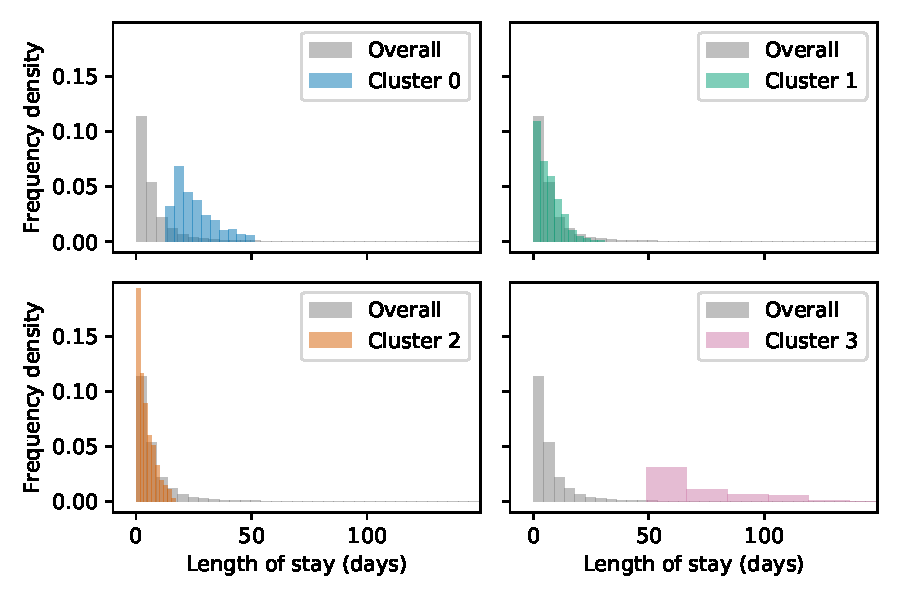
\includegraphics[width=\linewidth]{cluster_los}
        \caption{}\label{fig:cluster_los}
    \end{subfigure}\hfill%
    \begin{subfigure}{\halfimgwidth}
        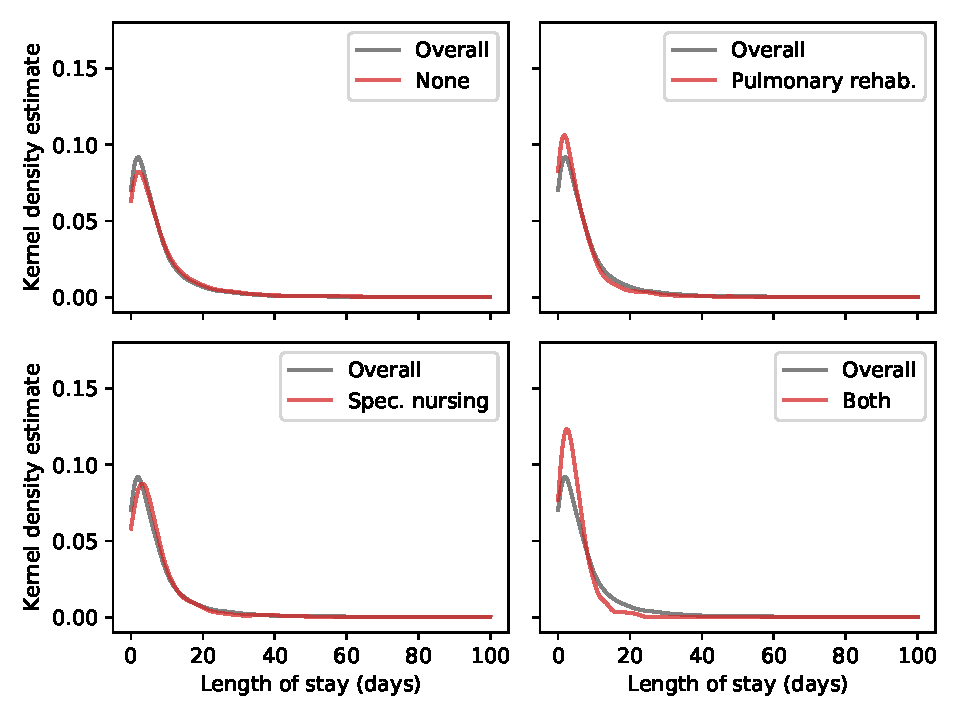
\includegraphics[width=\linewidth]{intervention_los}
        \caption{}\label{fig:intervention_los}
    \end{subfigure}
    \caption{%
        Kernel density estimate plots for length of stay by
        (\subref{fig:cluster_los}) cluster and (\subref{fig:intervention_los})
        intervention
    }\label{fig:los_kde}
\end{figure}

\begin{figure}
    \centering
    \begin{subfigure}{\halfimgwidth}
        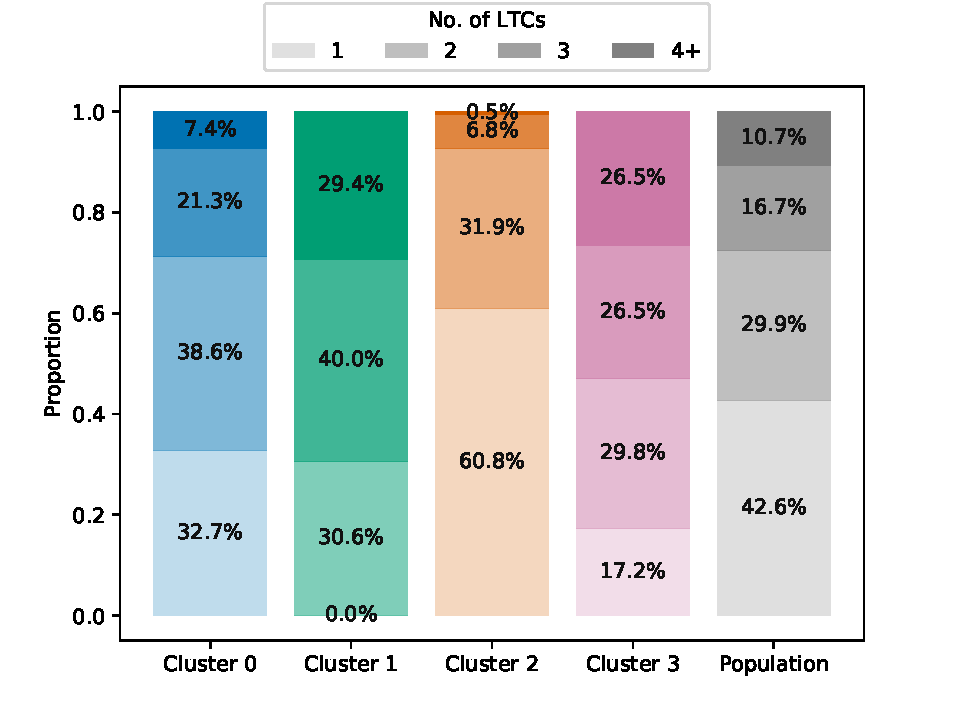
\includegraphics[width=\linewidth]{cluster_ltcs}
        \caption{}\label{fig:cluster_ltcs}
    \end{subfigure}\hfill%
    \begin{subfigure}{\halfimgwidth}
        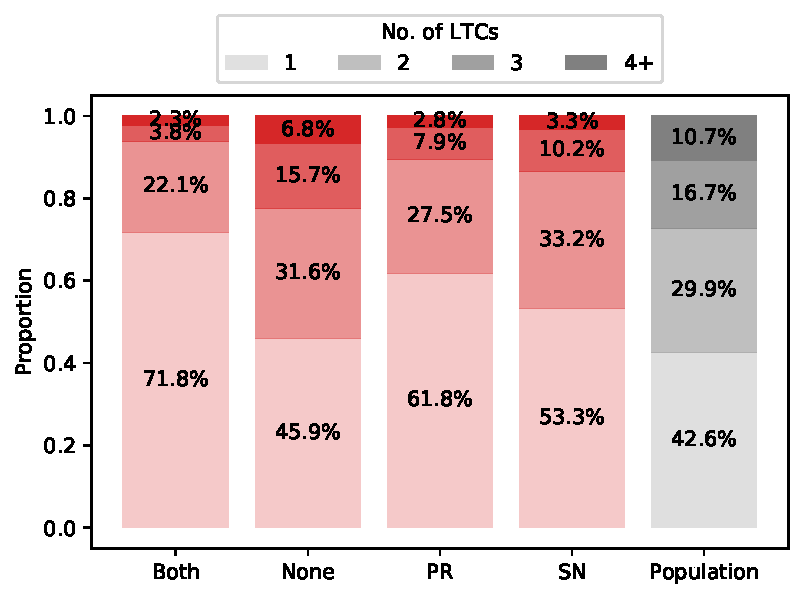
\includegraphics[width=\linewidth]{intervention_ltcs}
        \caption{}\label{fig:intervention_ltcs}
    \end{subfigure}
    \caption{%
        Proportions of concurrent LTC counts presented by patients by
        (\subref{fig:cluster_ltcs}) cluster and (\subref{fig:intervention_ltcs})
        intervention
    }\label{fig:ltcs}
\end{figure}

\begin{figure}
    \centering
    \begin{subfigure}{\halfimgwidth}
        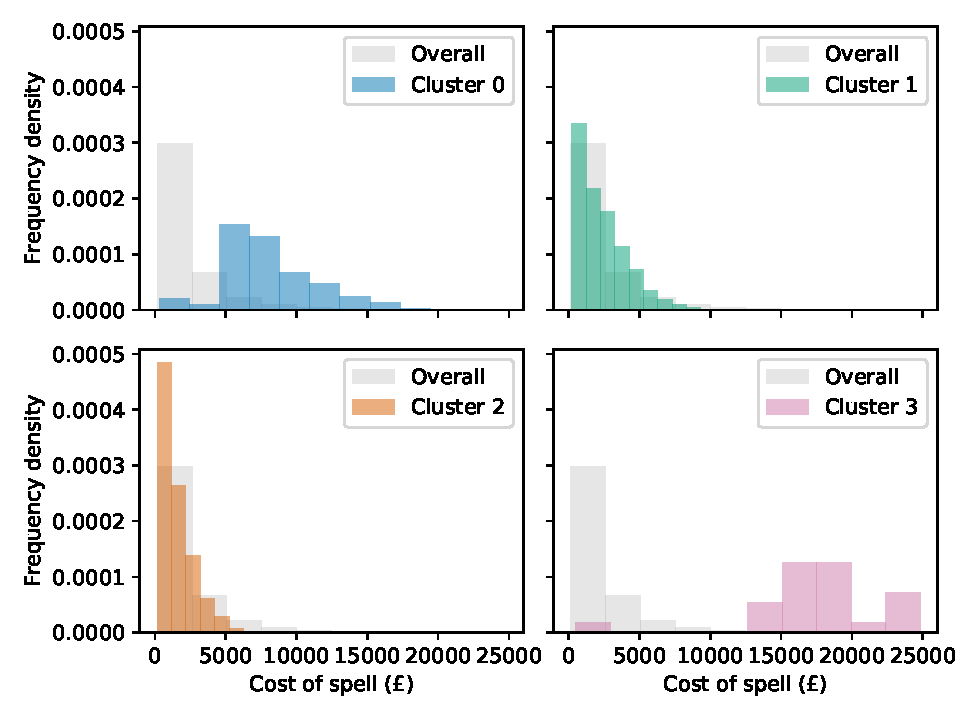
\includegraphics[width=\linewidth]{cluster_spell_cost}
        \caption{}\label{fig:cluster_spell_cost}
    \end{subfigure}\hfill%
    \begin{subfigure}{\halfimgwidth}
        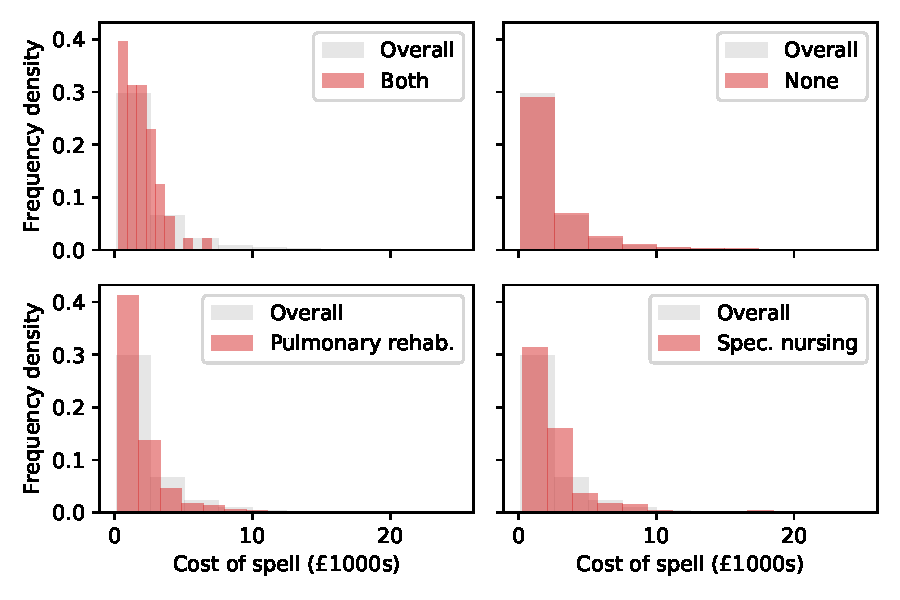
\includegraphics[width=\linewidth]{intervention_spell_cost}
        \caption{}\label{fig:intervention_spell_cost}
    \end{subfigure}
    \caption{%
        Histograms for spell costs by (\subref{fig:cluster_spell_cost}) cluster
        and (\subref{fig:intervention_spell_cost}) intervention
    }\label{fig:wimd_hist}
\end{figure}

\begin{figure}
    \centering
    \begin{subfigure}{\halfimgwidth}
        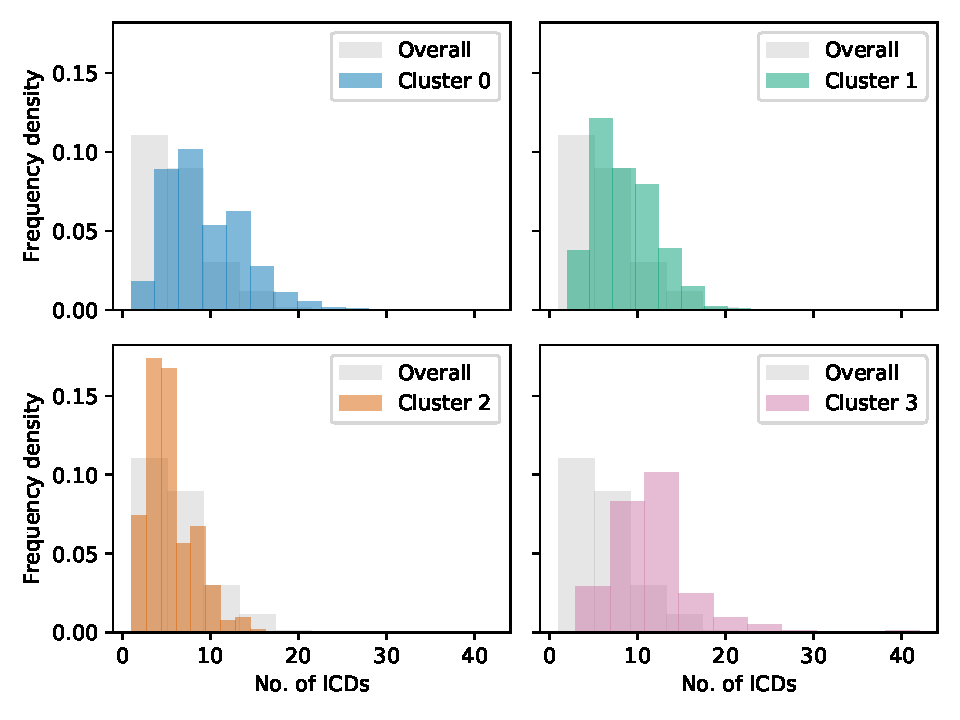
\includegraphics[width=\linewidth]{cluster_n_icds}
        \caption{}\label{fig:cluster_n_icds}
    \end{subfigure}\hfill%
    \begin{subfigure}{\halfimgwidth}
        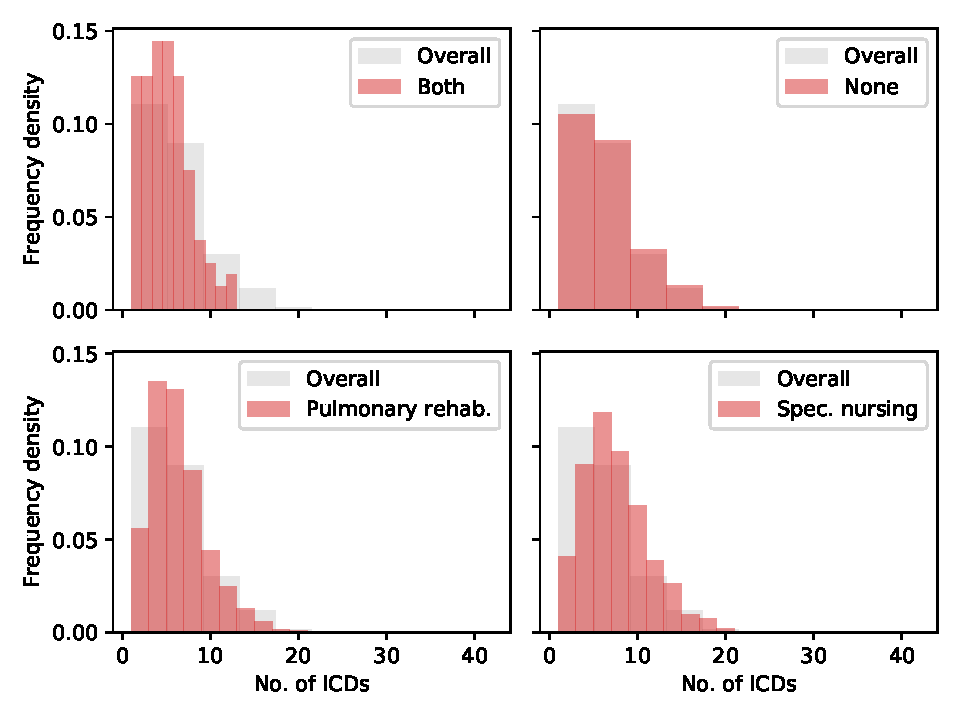
\includegraphics[width=\linewidth]{intervention_n_icds}
        \caption{}\label{fig:intervention_n_icds}
    \end{subfigure}
    \caption{%
        Histograms for number of ICDs by (\subref{fig:cluster_n_icds}) cluster
        and (\subref{fig:intervention_n_icds}) intervention
    }\label{fig:n_icds_hist}
\end{figure}

\begin{figure}
    \centering
    \begin{subfigure}{\halfimgwidth}
        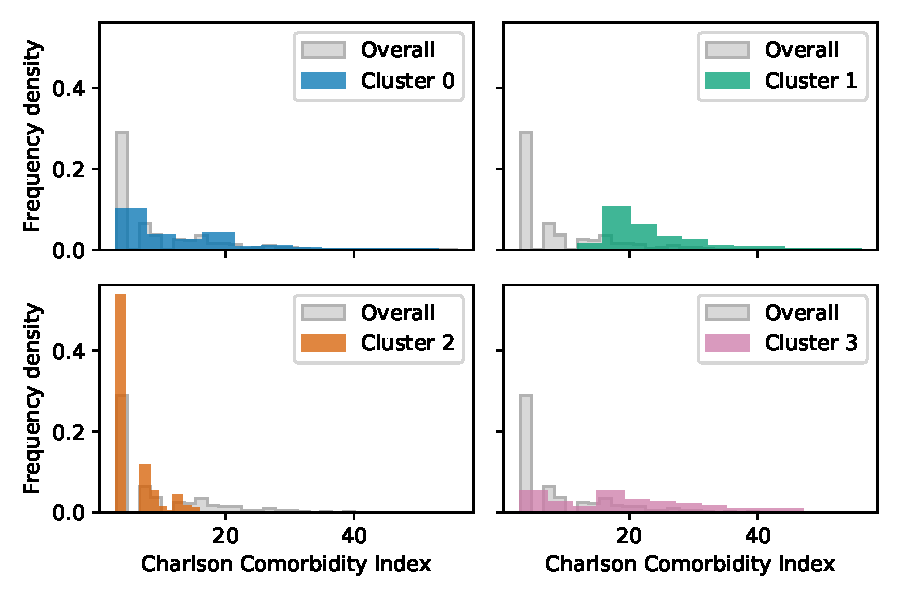
\includegraphics[width=\linewidth]{cluster_charlson_gross}
        \caption{}\label{fig:cluster_charlson}
    \end{subfigure}\hfill%
    \begin{subfigure}{\halfimgwidth}
        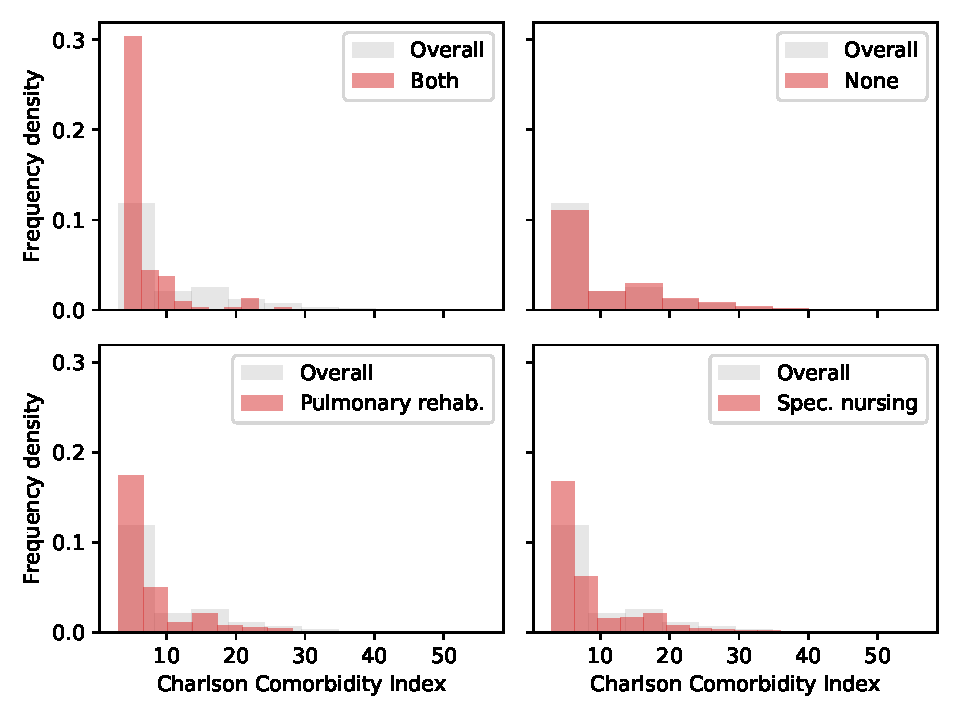
\includegraphics[width=\linewidth]{intervention_charlson_gross}
        \caption{}\label{fig:intervention_charlson}
    \end{subfigure}
    \caption{%
        Histograms for CCI by (\subref{fig:cluster_charlson}) cluster and
        (\subref{fig:intervention_charlson}) intervention
    }\label{fig:charlson_hist}
\end{figure}


% TODO Condensed analysis of clustering
%       - choosing k and a clustering algorithm
%       - comparison with treatment segmentation
